\documentclass[graphics]{beamer}
\usepackage[utf8]{inputenc}
\usepackage[french]{babel}
\usepackage{lmodern}
\usepackage{tcolorbox}
\usepackage{pgfpages}
\usepackage{graphicx}
\usepackage{mathdots}
\usepackage{subcaption}
\usepackage{xcolor}
\usepackage[export]{adjustbox}
\usepackage{appendixnumberbeamer}
\usepackage{stmaryrd} 
\usepackage{caption}
\usepackage{version}
\usepackage{nicematrix}
\captionsetup[figure]{labelformat=empty}

\newenvironment{changemargin}[2]{%
\begin{list}{}{%
\setlength{\topsep}{0pt}%
\setlength{\leftmargin}{#1}%
\setlength{\rightmargin}{#2}%
\setlength{\listparindent}{\parindent}%
\setlength{\itemindent}{\parindent}%
\setlength{\parsep}{\parskip}%
}%
\item[]}{\end{list}}



\usetheme{Warsaw}
\usecolortheme{dolphin}

\title[Weak Schur numbers]{Weak Schur numbers}
\subtitle{P05 - Formation à la recherche 1A}
\author[R. Ageron, P. Castéras, T. Pellerin, Y. Portella]{Romain Ageron, Paul Castéras, Thibaut Pellerin, Yann Portella}
\titlegraphic{\centering
	
\includegraphics[scale=.08]{cs}
}
%\institute[]{\'CentraleSupélec}
\date{3 juin 2021}
	\setbeamersize{text margin left=15pt}
	\setbeamersize{text margin right=15pt}


% pour supprimer les symboles de navigation
\setbeamertemplate{navigation symbols}{}
% \setbeamertemplate{footline}[frame number]
\setbeamertemplate{caption}{\raggedright\insertcaption\par}

\newcommand\blfootnote[1]{%
	\begingroup
	\renewcommand\thefootnote{}\footnote{#1}%
	\addtocounter{footnote}{-1}%
	\endgroup
}

\begin{document}

\begin{frame}
\titlepage
%\begin{center}
%	\includegraphics[height=0.5cm]{logoens.pdf}
%\end{center}
\end{frame}

\section{Présentation}
\subsection{Un~problème~de~partition}
\begin{frame}
	En 1917, le russe \textbf{Issai Schur} pose le problème suivant :
	\pause
	\begin{itemize}
		\item Pour \(n \geq 1\) un entier
		\item Et \(k \geq 1\) un autre entier ( = nombre de \textbf{couleurs})
	\end{itemize}
	\pause
	\begin{tcolorbox}[colback=green!5,colframe=green!40!black,title=Question]
		Peut-on colorier les entiers de \(1\) à \(n\) de sorte que si deux nombres ont la même couleur,
		leur somme n'est pas de cette couleur ? Si oui, un tel coloriage est dit \textbf{sans sommes}.
	\end{tcolorbox}
\end{frame}

\subsection{Les~nombres~de~Schur}

\begin{frame}
	Pour \(n = 13\) et \(k = 3\), le coloriage \\
	\begin{center}
	\begin{NiceTabular}{|*{13}{c|}}[standard-cline,hlines]
		\CodeBefore
			\cellcolor{red}{1-1}
			\cellcolor{cyan}{1-2}
			\cellcolor{cyan}{1-3}
			\cellcolor{red}{1-4}
			\cellcolor{green}{1-5}
			\cellcolor{green}{1-6}
			\cellcolor{cyan}{1-7}
			\cellcolor{green}{1-8}
			\cellcolor{green}{1-9}
			\cellcolor{red}{1-10}
			\cellcolor{cyan}{1-11}
			\cellcolor{cyan}{1-12}
			\cellcolor{red}{1-13}
		\Body
			1 & 2 & 3 & 4 & 5 & 6 & 7 & 8 & 9 & 10 & 11 & 12 & 13\\
	\end{NiceTabular}
	\end{center}
	vérifie cette propriété.
	\pause
	\begin{tcolorbox}[colback=red!5,colframe=red!40!black,title=Définition]
		Pour \(k\) couleurs, on note \(S(k)\) le plus grand entier \(n\) tel qu'on puisse colorier les entiers de
		\(1\) à \(n\) en vérifiant cette propriété. C'est le \(k\)-ième \textbf{nombre de Schur}.
	\end{tcolorbox}
	\pause
	Sur l'exemple, on peut vérifier que \(S(3) = 13\) : on ne peut colorier \([\![1,14]\!]\) avec trois couleurs.
\end{frame}

\subsection{Weak~Schur}

\begin{frame}
	\begin{tcolorbox}[colback=red!5,colframe=red!40!black,title=Définition]
		Un coloriage est dit \textbf{faiblement sans sommes} lorsque pour deux nombres \textbf{différents} de même couleur,
		leur somme n'est pas de la même couleur. On définit avec cette propriété \(WS(k)\), le \(k\)-ième 
		\textbf{nombre de Schur faible}.
	\end{tcolorbox}
	\pause
	Un coloriage sans sommes et en particulier faiblement sans somme, donc on a toujours \(WS(k) \geq S(k)\).\\
	\pause 
	\begin{center}
	\begin{NiceTabular}{|*{4}{c|}}[standard-cline,hlines]
		\CodeBefore
			\cellcolor{red}{1-1}
			\cellcolor{cyan}{1-2}
			\cellcolor{cyan}{1-3}
			\cellcolor{red}{1-4}
		\Body
			1 & 2 & 3 & 4 \\
	\end{NiceTabular}

	\begin{NiceTabular}{|*{8}{c|}}[standard-cline,hlines]
		\CodeBefore
			\cellcolor{red}{1-1}
			\cellcolor{red}{1-2}
			\cellcolor{cyan}{1-3}
			\cellcolor{red}{1-4}
			\cellcolor{cyan}{1-5}
			\cellcolor{cyan}{1-6}
			\cellcolor{cyan}{1-7}
			\cellcolor{red}{1-8}
		\Body
			1 & 2 & 3 & 4 & 5 & 6 & 7 & 8 \\
	\end{NiceTabular}
	\end{center}
	\(S(2) = 4\) mais \(WS(2) = 8\)
\end{frame}

\section{L'état~de~l'art}
\subsection{Calculer~ces~nombres}

\begin{frame}
	\begin{itemize}
	\item Pour montrer que \(S(k) = n\), il faut : 
	\begin{itemize} 
		\item trouver un coloriage sans sommes de \([\![1,n]\!]\) à \(k\) couleurs
		\item montrer qu'on ne peut pas colorier \([\![1,n+1]\!]\). 
	\end{itemize}
	\pause
	\item En pratique, on se contente de \textbf{minorer} \(S(k)\) :
	\begin{itemize}
	\item inégalités récursives 
	\item recherche de coloriages par ordinateur
	\end{itemize}
	\end{itemize}
\end{frame}

\subsection{Approche~numérique}

\begin{frame}
	Les recherches récentes sur le sujet se focalisent sur les méthodes numériques.
	\begin{itemize}
		\item On fixe \(k\) et on essaye de colorier le plus loin possible
		\item Plusieurs façon d'encoder le problème :
		\begin{itemize}
		\item arbre \(\rightarrow\) \textbf{Monte-Carlo Tree Search} sur un espace de recherche restreint
		\item formules booléennes \(\rightarrow\) solveur \textbf{SAT} 
		\end{itemize}
		\pause
		\item Améliorations des bornes inférieures pour \(k \geq 5\) 
		\item Temps de calcul : le calcul exact de \(S(5)\) via un solveur SAT a demandé 20 années de calcul machine !
	\end{itemize}
	
\end{frame}

\section{Amélioration~des~nombres~de~Schur}
\subsection{Un~article~fondateur~:~Abbott~et~Hanson}
\begin{frame}
La borne inférieure établie par I. Schur est :
\[S(n+1) \geqslant 3S(n) + 1 \Longrightarrow S(n) \geqslant \frac{3^n - 1}{2}
\]
Une première piste pour améliorer cette borne est proposée par H. L. Abbott et D. Hanson en 1972. Ils prouvent :
\[
S(n+m) \geqslant S(n) \left( 2S(m) + 1 \right) + S(m)
\]
Que font-ils concrètement ?
\end{frame}
\begin{frame}
Un exemple pour \(n = m = 2\) :
\renewcommand{\arraystretch}{1.7}
\begin{center}
\begin{NiceTabular}{|*{9}{c|}}[corners=SE,standard-cline,hlines]
\CodeBefore
	\cellcolor{red}{1-1}
	\cellcolor{green}{1-2}
	\cellcolor{green}{1-3}
	\cellcolor{red}{1-4}
	\cellcolor{cyan}{1-5}
	\cellcolor{cyan}{1-6}
	\cellcolor{cyan}{1-7}
	\cellcolor{cyan}{1-8}
	\cellcolor{cyan}{1-9}
	\cellcolor{red}{2-1}
	\cellcolor{green}{2-2}
	\cellcolor{green}{2-3}
	\cellcolor{red}{2-4}
	\cellcolor{yellow}{2-5}
	\cellcolor{yellow}{2-6}
	\cellcolor{yellow}{2-7}
	\cellcolor{yellow}{2-8}
	\cellcolor{yellow}{2-9}
	\cellcolor{red}{3-1}
	\cellcolor{green}{3-2}
	\cellcolor{green}{3-3}
	\cellcolor{red}{3-4}
	\cellcolor{yellow}{3-5}
	\cellcolor{yellow}{3-6}
	\cellcolor{yellow}{3-7}
	\cellcolor{yellow}{3-8}
	\cellcolor{yellow}{3-9}
	\cellcolor{red}{4-1}
	\cellcolor{green}{4-2}
	\cellcolor{green}{4-3}
	\cellcolor{red}{4-4}
	\cellcolor{cyan}{4-5}
	\cellcolor{cyan}{4-6}
	\cellcolor{cyan}{4-7}
	\cellcolor{cyan}{4-8}
	\cellcolor{cyan}{4-9}
	\cellcolor{red}{5-1}
	\cellcolor{green}{5-2}
	\cellcolor{green}{5-3}
	\cellcolor{red}{5-4}
\Body
	1 & 2 & 3 & 4 & 5 & 6 & 7 & 8 & 9 \\
	10 & 11 & 12 & 13 & 14 & 15 & 16 & 17 & 18 \\
	19 & 20 & 21 & 22 & 23 & 24 & 25 & 26 & 27 \\
	28 & 29 & 30 & 31 & 32 & 33 & 34 & 35 & 36 \\
	37 & 38 & 39 & 40 \\
	
\end{NiceTabular}
\end{center}
\[S(4) \geqslant S(2) \left( 2S(2) + 1 \right) + S(2) = 40
\]
\end{frame}
\subsection{Une~extension~:~les~SF-templates}
\begin{frame}
\begin{itemize}
\item F. Rowley améliore cette approche théorique en 2020.
\pause
\item \textbf{Extension verticale} de structures plus générales : les SF-templates.
\pause
\item \textbf{Notre contribution} : recherche de SF-templates intéressants
\pause
\item Recette : SF-template = Partition sans somme + condition suivante :
\[
\forall i \in [\![1, n-1]\!], \forall (x,y) \in A_i^2, x+y > p
\Longrightarrow x+y-p \notin A_i
\]
\end{itemize}
\end{frame}
\begin{frame}
En fait, l'exemple précédent faisait déjà apparaître un SF-template, en voici un autre :
\begin{center}
\renewcommand{\arraystretch}{1.7}
\begin{NiceTabular}{|*{9}{c|}}[corners=SE,standard-cline,hlines]
\CodeBefore
	\cellcolor{red}{1-1}
	\cellcolor{green}{1-2}
	\cellcolor{green}{1-3}
	\cellcolor{red}{1-4}
	\cellcolor{cyan}{1-5}
	\cellcolor{cyan}{1-6}
	\cellcolor{red}{1-7}
	\cellcolor{cyan}{1-8}
	\cellcolor{cyan}{1-9}
	\cellcolor{red}{2-1}
	\cellcolor{green}{2-2}
	\cellcolor{green}{2-3}
	\cellcolor{red}{2-4}
	\cellcolor{yellow}{2-5}
	\cellcolor{yellow}{2-6}
	\cellcolor{red}{2-7}
	\cellcolor{yellow}{2-8}
	\cellcolor{yellow}{2-9}
	\cellcolor{red}{3-1}
	\cellcolor{green}{3-2}
	\cellcolor{green}{3-3}
	\cellcolor{red}{3-4}
	\cellcolor{yellow}{3-5}
	\cellcolor{yellow}{3-6}
	\cellcolor{red}{3-7}
	\cellcolor{yellow}{3-8}
	\cellcolor{yellow}{3-9}
	\cellcolor{red}{4-1}
	\cellcolor{green}{4-2}
	\cellcolor{green}{4-3}
	\cellcolor{red}{4-4}
	\cellcolor{cyan}{4-5}
	\cellcolor{cyan}{4-6}
	\cellcolor{red}{4-7}
	\cellcolor{cyan}{4-8}
	\cellcolor{cyan}{4-9}
	\cellcolor{red}{5-1}
	\cellcolor{green}{5-2}
	\cellcolor{green}{5-3}
	\cellcolor{red}{5-4}
\Body
	1 & 2 & 3 & 4 & 5 & 6 & 7 & 8 & 9 \\
	10 & 11 & 12 & 13 & 14 & 15 & 16 & 17 & 18 \\
	19 & 20 & 21 & 22 & 23 & 24 & 25 & 26 & 27 \\
	28 & 29 & 30 & 31 & 32 & 33 & 34 & 35 & 36 \\
	37 & 38 & 39 & 40 \\
\end{NiceTabular}
\end{center}
\vspace{1ex}
\renewcommand{\arraystretch}{1.7}
\begin{center}
\begin{NiceTabular}{|*{9}{c|}}[standard-cline,hlines]
	\CodeBefore 
		\cellcolor{red}{1-1}
		\cellcolor{green}{1-2}
		\cellcolor{green}{1-3}
		\cellcolor{red}{1-4}
		\cellcolor{cyan}{1-5}
		\cellcolor{cyan}{1-6}
		\cellcolor{red}{1-7}
		\cellcolor{cyan}{1-8}
		\cellcolor{cyan}{1-9}
	\Body
		1 & 2 & 3 & 4 & 5 & 6 & 7 & 8 & 9 \\
\end{NiceTabular}
\end{center}
\end{frame}
\subsection{Nouvelles~bornes}
\begin{frame}
\begin{changemargin}{-0.7cm}{-0.7cm}
\begin{center}
Quelques résultats !
\[
\begin{array}{c}
	\begin{NiceArray}{cwc{8ex}wc{10ex}wc{10ex}wc{11ex}}[hvlines]
	\CodeBefore
		\cellcolor{yellow}{2-2}
		\cellcolor{yellow}{3-3}
		\cellcolor{yellow}{4-4}
		\cellcolor{yellow}{4-5}
	\Body
		n & 8 & 9 & 10 & 11 \\
		33 \, S(n-3) + 6 & 5\,286 & 17\,694 & 55\,446 & 174\,444 \\
		111 \, S(n-4) + 43 & 4927 & 17\,803 & 59\,539 & 186\,523 \\
		380 \, S(n-5) + 148 & 5\,088 & 16\,868 & 60\,948 & 203\,828 \\
		1\,140 \, S(n-6) + 528 & 5\,088 & 15\,348 & 50\,688 & 182\,928 \\
	\end{NiceArray}
	\\ \\
	\begin{NiceArray}{cwc{8ex}wc{10ex}wc{10ex}wc{11ex}}[hvlines]
	\CodeBefore
		\cellcolor{yellow}{2-3}
		\cellcolor{yellow}{4-2}
		\cellcolor{yellow}{4-4}
		\cellcolor{yellow}{4-5}
	\Body
		n & 12 & 13 & 14 & 15 \\
		33 \, S(n-3) + 6 & 587\,505 & 2\,011\,290 & 6\,726\,330 & 21\,072\,090 \\
		111 \, S(n-4) + 43 & 586\,789 & 1\,976\,176 & 6\,765\,271 & 22\,624\,951 \\
		380 \, S(n-5) + 148 & 638\,548 & 2\,008\,828 & 6\,765\,288 & 23\,160\,388 \\
		1\,140 \, S(n-6) + 528 & 611\,568 & 1\,915\,728 & 6\,026\,568 & 20\,295\,948 \\
	\end{NiceArray}
\end{array}
\]

\end{center}
\end{changemargin}
\end{frame}

\section{Template~pour~les~nombres~de~Weak~Schur}


\subsection{Inégalités~entre~les~nombres~de~Schur~et~de~Weak~Schur}


\begin{frame}
	\begin{itemize}
		\item \textbf{Premières inégalités obtenues par Rowley:}
		\vspace{3 mm}
			\begin{itemize}
			\item $WS(n+1) \geqslant 4S(n)+2$
			\item $WS(n+2) \geqslant 13S(n)+8$
			\end{itemize}
		\vspace{5 mm}
		\item \textbf{Notre inégalité généralisée:} 
		\vspace{5 mm} Soit $(n,k) \in \mathbb{N}^2$,
			\fbox{$WS (n+k) \geqslant S(k) \left (WS (n) + \left \lceil 					\displaystyle \frac{WS (n)}{2}
			\right \rceil +1 \right) + WS (n)$}
	\end{itemize}
\end{frame}

\begin{frame}
\begin{center}
$WS (n+k) \geqslant S(k) \left (WS (n) +\left \lceil \displaystyle \frac{WS (n)}{2}
			\right \rceil +1 \right) + WS (n)$
\end{center}

\begin{figure}
        \centering
        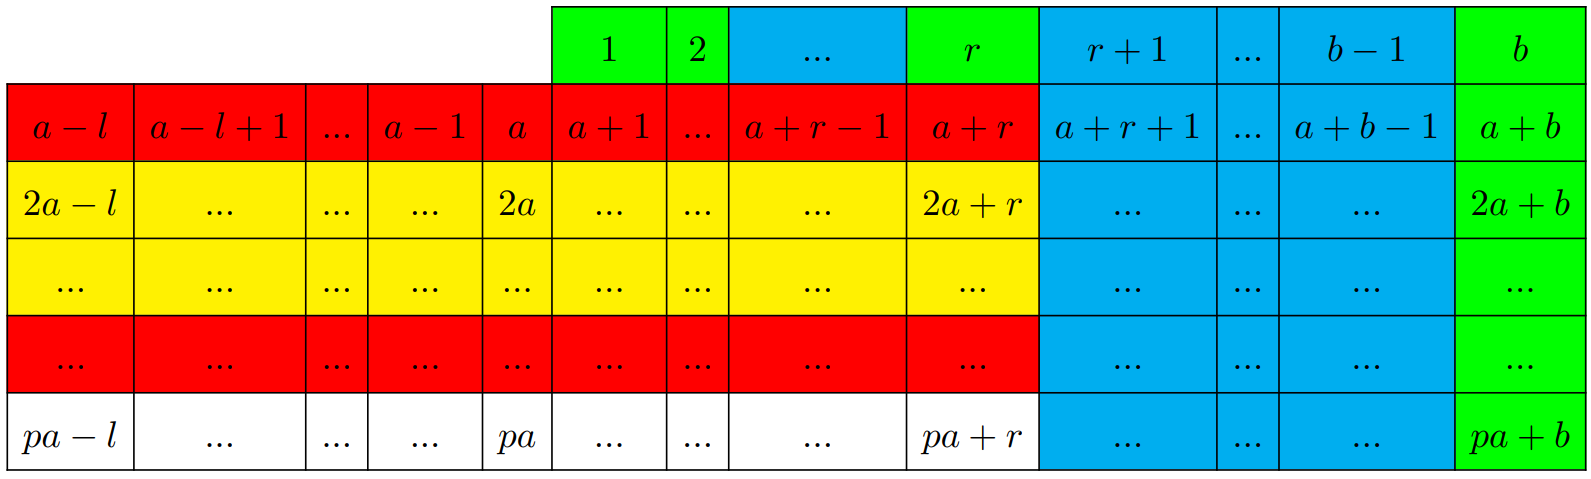
\includegraphics[scale=0.7]{tableau.png}
\end{figure}
\end{frame}

\subsection{Principe~général~du~template~Weak~Schur}
\begin{frame}


\begin{itemize}
\item On cherche un template à n couleurs de cardinal $WS^+(n)$ tel que:
\newline $WS(n+k) \geqslant S(k)WS^+(n)+b$
\vspace{8 mm}
\item Or $WS (n+k) \geqslant S(k) \left (WS (n) + \left \lceil 					\displaystyle \frac{WS (n)}{2}
			\right \rceil +1 \right) + WS (n)$
			\vspace{8 mm}
\item Par conséquent, $WS^+(n) \geqslant WS (n) + \left \lceil 					\displaystyle \frac{WS (n)}{2}
			\right \rceil +1 $
\end{itemize}

\end{frame}

\subsection{Nouvelles~valeurs~obtenus}

\begin{frame}
\begin{figure}
        \centering
        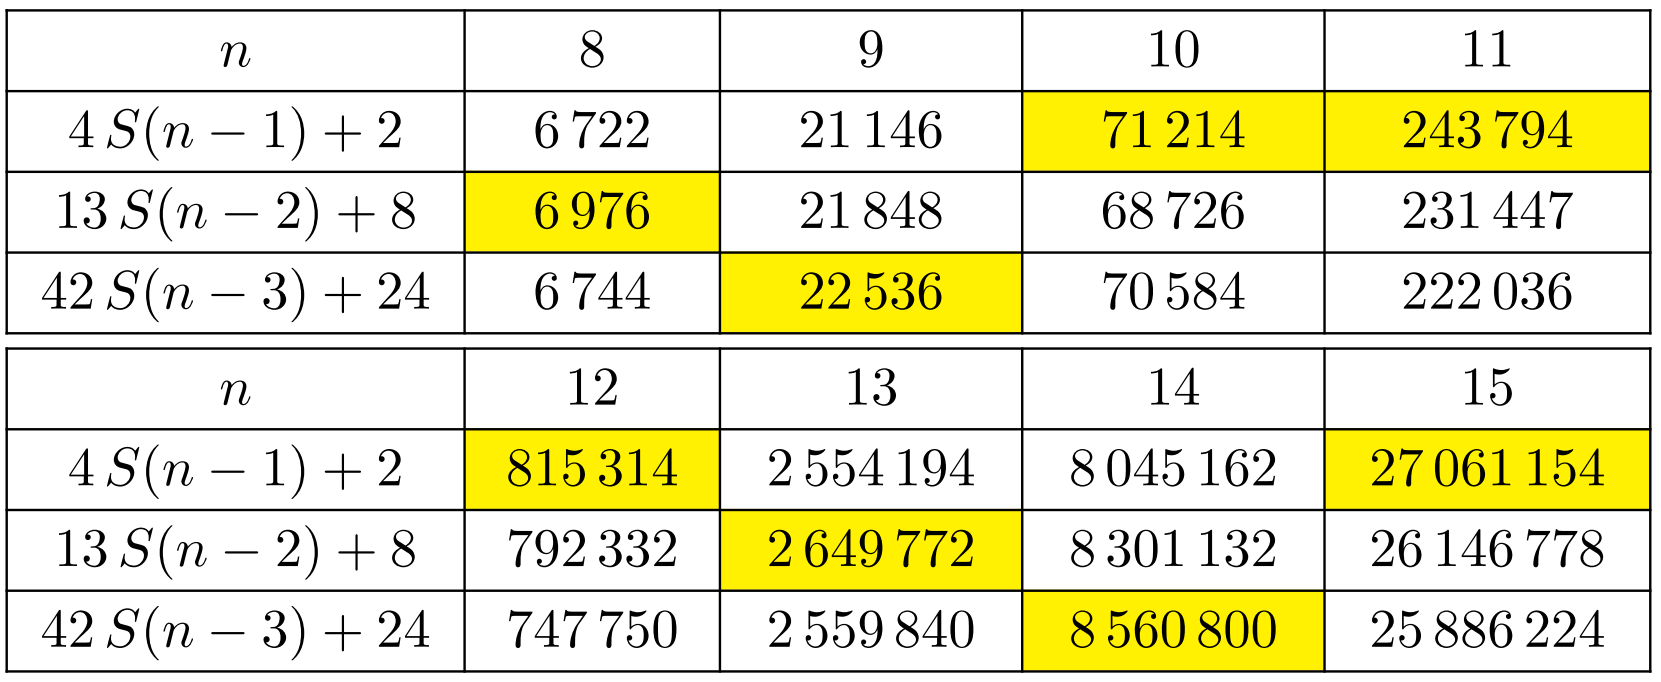
\includegraphics[scale=0.30]{tableau_resultat.png}
\end{figure}

\end{frame}
\end{document}